% Found in Transliteration: Closing the Script Gap in Hindi/Gujarati Retrieval
% Compile with XeLaTeX (Overleaf: Menu -> Compiler -> XeLaTeX), then BibTeX, then XeLaTeX twice.
% Tables and figures in generated/ are copies of results/ made by
%   python -m scripts.build_report_assets --config configs/report.yaml
% and every metric value in the text is checked against results/ by
%   python -m scripts.check_report_numbers --config configs/report.yaml
\documentclass[11pt,a4paper]{article}

\usepackage[margin=2.2cm]{geometry}
\usepackage{fontspec}
\usepackage{amsmath,amssymb}
\usepackage{booktabs}
\usepackage{graphicx}
\usepackage{xcolor}
\usepackage[font=small,labelfont=bf]{caption}
\usepackage{float}
\usepackage[numbers,sort&compress]{natbib}
\usepackage[hidelinks]{hyperref}

% Native-script examples: Devanagari and Gujarati need OpenType fonts that cover them.
\newfontfamily\devfont{Noto Sans Devanagari}[Script=Devanagari]
\newfontfamily\gujfont{Noto Sans Gujarati}[Script=Gujarati]
\newcommand{\dev}[1]{{\devfont #1}}
\newcommand{\guj}[1]{{\gujfont #1}}
\newcommand{\rom}[1]{\texttt{#1}}          % a romanized query or word, as typed
\newcommand{\gr}{\mathrm{GapRecovered}}

\title{Found in Transliteration:\\ Closing the Script Gap in Hindi and Gujarati Retrieval}
\author{% Fill in the author block.
}
\date{Information Retrieval course project, DA-IICT}

\begin{document}
\maketitle

\begin{abstract}
People in India often type Hindi and Gujarati in Latin script (\rom{kisan andolan news}),
while the documents they want are written in the native script (\dev{किसान आंदोलन}). The
query and the documents then share no characters. We reproduce this \emph{script gap} on
MIRACL-hi: with romanized queries, nDCG@10 drops by 99.6\% for BM25 and by 97.8\% for a
multilingual dense retriever (e5-base), the same near-total collapse a recent SIGIR paper
reports for Chinese. We then compare four ways to close the gap: back-transliterating the
query, normalizing spelling variants on both sides or romanizing the index, fine-tuning the
dense model on romanized queries, and fusing lexical and dense runs. Back-transliteration is
the key step: with the unchanged dense model it recovers 92\% of the gap. Fine-tuning on
1,168 romanized queries recovers 36\%. Interpolating normalized BM25 with dense retrieval
reaches nDCG@10 0.6115 on natural romanized queries, 101\% of the gap and level with dense
retrieval on the original native queries. The same recipe, re-tuned on Gujarati, recovers
110\% of the gap there, and the ranking of methods largely carries over. What remains is
transliteration error, not code-mixing or query length.
\end{abstract}

% ===========================================================================
\section{Introduction}

Hindi and Gujarati are written in their own scripts (Devanagari and Gujarati), but on phones
and laptops many users type them in Latin letters, in an informal ``Hinglish'' spelling: there
is no standard, so the same word appears as \rom{mein}, \rom{me} or \rom{men}. A search
engine whose documents are in native script then sees a query that shares no characters with
any document. Lexical retrievers such as BM25 match nothing, and, as we show, multilingual
dense retrievers lose most of their quality as well.

\citet{chari2025lost} call this drop the \emph{script gap} and measure it for Chinese and
Russian with a dense retriever and a reranker. They close part of it by fine-tuning on
romanized training queries (``transliterate-train''). Their study has no lexical baseline and
tests only one way of closing the gap. We ask four questions, for Hindi as the core language
and Gujarati as a second one:

\begin{enumerate}
  \item How large is the script gap for lexical and dense retrieval on Hindi, with romanized
        queries written the way people type them?
  \item Which approach closes it best: rewriting the query into native script,
        normalizing the documents, fine-tuning the dense model, or fusing methods?
  \item What causes the gap that remains?
  \item Does the answer carry over to Gujarati?
\end{enumerate}

\paragraph{Contributions.}
(i) A reproduction of the script gap on Hindi with three kinds of romanized queries: an LLM's
casual romanization (our main condition), the rule-based Uroman romanization used by
\citet{chari2025lost}, and 50 queries romanized by hand. (ii) A comparison of four families of
gap-closing methods on the same data, always next to the baselines, with every setting chosen
on a separate tune split. (iii) A hybrid of normalized BM25 and dense retrieval, both on the
back-transliterated query, that closes the whole gap on natural romanized queries. (iv) An
error analysis of what remains, and a transfer study to Gujarati. (v) A side-by-side search
demo. All code, configurations and per-query results are in the project repository.

% ===========================================================================
\section{Related work}

\paragraph{The script gap in neural IR.}
\citet{chari2025lost} romanize mMARCO and neuCLIR queries in Chinese and Russian with Uroman
\citep{hermjakob2018uroman} and search native documents with BGE-M3 and an mT5 reranker. With
romanized queries, BGE-M3's MRR@10 on Chinese drops from 0.2342 to 0.0078 (97\%), and on
Russian, whose script shares letters with Latin, by 49\% (their Table 1). Fine-tuning on a
half-native, half-romanized training set (their configuration ``50'') makes the models robust
while keeping native performance in domain, but costs native performance out of domain (their
Table 2). They do not report a lexical baseline, and their romanized queries are
machine-generated. We follow their setup (native documents, the same queries in two scripts,
the N/50/T fine-tuning configurations, Bonferroni-corrected tests) on Hindi, and add lexical
baselines, natural and hand-typed romanizations, and query- and document-side methods.

\paragraph{Mixed-script and transliterated search.}
Searching with romanized Indian-language queries has been studied before neural retrieval,
e.g.\ query expansion for mixed-script retrieval \citep{gupta2014query} and the shared tasks
on mixed-script IR at FIRE. Romanized Indic text has also been collected at scale: the
Dakshina dataset pairs native and romanized sentences \citep{roark2020dakshina}, and
Aksharantar provides transliteration pairs and the IndicXlit models we use to
back-transliterate queries \citep{madhani2023aksharantar}.

\paragraph{Retrieval components.}
We use BM25 \citep{robertson2009bm25} through PyTerrier \citep{macdonald2020pyterrier},
multilingual-e5-base as the dense retriever \citep{wang2024me5}, contrastive fine-tuning with
an InfoNCE loss \citep{oord2018infonce,karpukhin2020dpr}, and reciprocal rank fusion
\citep{cormack2009rrf} as well as score interpolation for hybrids. The collections are
MIRACL \citep{zhang2022miracl} for Hindi and IndicQA \citep{doddapaneni2023indicxtreme} with
Wikipedia distractors for Gujarati; evaluation uses \texttt{ir\_measures}
\citep{macavaney2022irmeasures}.

% ===========================================================================
\section{Data}

\subsection{Hindi: MIRACL-hi}
MIRACL-hi \citep{zhang2022miracl} has 506,264 passages of Hindi Wikipedia, and questions
written and judged by native speakers. Only its \texttt{dev} split has public judgments, so we
split it with a fixed seed into 100 \emph{tune} queries (every parameter choice) and 250
\emph{test} queries (final numbers only). The 1,168 \texttt{train} queries are used only for
fine-tuning; one train query that repeats a test question under another id was removed. About
10 passages per query are judged, about 2 of them relevant. All statistics are computed by a
script and recorded in the project's data card.

\subsection{Romanized query sets}
Every query exists in four versions with the same id:
\begin{itemize}
  \item \textbf{native}: the original Devanagari question;
  \item \textbf{natural} (main condition): written by an LLM (Gemini, temperature 0) as a
        typical user would type it, e.g.\ \rom{kisan andolan ki taza khabar}; generated once and
        frozen;
  \item \textbf{rule}: Uroman, called exactly as in the reference paper's code, e.g.\
        \rom{raajaa raamamohan raay}; deterministic but unlike real typing;
  \item \textbf{human}: 50 test queries romanized by hand, as a realism check.
\end{itemize}
Measured against the hand-typed queries, the natural set has a character error rate of 0.096
and the rule set 0.236: the natural set is much closer to real typing, though not identical.
The natural set spells English words and well-known names the English way (\rom{cricket},
\rom{delhi}), as users do.

\subsection{Gujarati: IndicQA-gu with Wikipedia distractors}
MIRACL has no Gujarati. The Gujarati part of IndicQA \citep{doddapaneni2023indicxtreme}, as
packaged for retrieval by MTEB, has native Gujarati questions over Gujarati Wikipedia
paragraphs, but only 248 judged passages, each answering several questions. Retrieval over
248 passages would be close to trivial, so we add unjudged distractors from the Gujarati
Wikipedia dump. Articles that share a word 8-gram with a judged passage are dropped (they may
contain a copy of it), the rest is cut into passages of 130--300 words to match the judged
passages' median length, and mostly-English passages and exact repeats are removed. The
collection has 51,129 passages. We sample 100 tune and 500 test queries (seed 42) and create
natural and rule romanizations with the Hindi procedure. Each query has exactly one relevant
passage, and there is no training split.

% ===========================================================================
\section{Methods}

\subsection{Baselines}
\textbf{BM25} scores a passage $d$ for a query $q$ as
\begin{equation}
  \mathrm{BM25}(q,d) = \sum_{t \in q} \mathrm{IDF}(t)\,
  \frac{tf_{t,d}\,(k_1+1)}{tf_{t,d} + k_1\left(1 - b + b\,\frac{|d|}{\mathrm{avgdl}}\right)},
\end{equation}
with $k_1$ and $b$ tuned on the tune split ($k_1 = 1.2$, $b = 0.3$ for Hindi; $1.5$ and $0.6$
for Gujarati). We index title and text with a Unicode tokenizer, without stemming or stop
words, and floor the IDF at 0, which drops terms that occur in more than half of the passages
(common Hindi function words such as \dev{के} otherwise get negative weights).

\textbf{Dense retrieval} uses multilingual-e5-base \citep{wang2024me5}, off the shelf, with
exact inner-product search over the whole corpus and passages cut at 256 tokens. For Gujarati
we compared 256 and 512 tokens on tune (nDCG@10 0.4358 and 0.3908) and kept 256.

\subsection{Query-side back-transliteration}
IndicXlit \citep{madhani2023aksharantar} turns each romanized word $w$ into up to ten native
candidates $c_{w,1},\dots,c_{w,10}$ with scores $s_{w,j}$ (its rescoring:
$0.9$ times the beam probability plus $0.1$ times a corpus word frequency). \textbf{Top-1}
replaces every word by its best candidate. The \textbf{weighted top-$k$} query keeps $k$
candidates per word with renormalized weights,
\begin{equation}
  q' = \bigcup_{w \in q} \left\{\left(c_{w,j},\, p_{w,j}\right)\right\}_{j=1}^{k},
  \qquad p_{w,j} = \frac{s_{w,j}}{\sum_{i=1}^{k} s_{w,i}},
\end{equation}
so each word contributes total weight 1 to the BM25 query ($k = 5$ for Hindi and $k = 3$ for
Gujarati, chosen on tune). The dense model receives the top-1 query.

\subsection{Document-side normalization and romanized indexes}
Many failures of back-transliteration are not errors but a different valid spelling: the
passage writes \dev{आरम्भिक}, IndicXlit returns \dev{आरंभिक}. A \textbf{normalization key}
maps such variants to one form on both sides: chandrabindu to anusvara, a nasal consonant
with virama before a consonant of its own class to anusvara, and Devanagari digits to ASCII
digits (three rules kept by a leave-one-out ablation on tune). For Gujarati the same rules
were rebuilt by shifting the characters into the Gujarati Unicode block. The opposite
direction is a \textbf{romanized index}: the passages are romanized with Uroman, a key of 11
rules maps Uroman and user spellings together (e.g.\ doubled letters, long vowels, schwa
deletion), and character 4-grams match near-misses. The \textbf{dual index} fuses the
native and the romanized route.

\subsection{Fine-tuning the dense retriever}
Following \citet{chari2025lost}, we fine-tune e5-base on the 1,168 training queries in three
configurations: native queries only (N), half native and half romanized (50), and romanized
only (T), always against native passages. The loss is InfoNCE with in-batch negatives and
judged non-relevant MIRACL passages as hard negatives,
\begin{equation}
  \mathcal{L} = -\log \frac{e^{s(q,d^+)/\tau}}
  {e^{s(q,d^+)/\tau} + \sum_{d^- \in \mathcal{N}(q)} e^{s(q,d^-)/\tau}},
\end{equation}
with $s$ the cosine similarity and $\tau = 0.01$. Checkpoints were chosen on tune.

\subsection{Hybrid fusion}
Hybrids combine a lexical and a dense run. Reciprocal rank fusion \citep{cormack2009rrf}
scores
\begin{equation}
  \mathrm{RRF}(d) = \sum_{r \in R} \frac{1}{k + \mathrm{rank}_r(d)},
\end{equation}
and score interpolation combines min-max normalized scores,
\begin{equation}
  \mathrm{score}(d) = \alpha\, \hat{s}_{\mathrm{lex}}(d) + (1-\alpha)\, \hat{s}_{\mathrm{dense}}(d),
  \qquad \hat{s}(d) = \frac{s(d) - \min s}{\max s - \min s},
\end{equation}
over the top 1000 of each run (a passage missing from a run gets 0 from it). Our final
system, \textbf{hybrid A}, interpolates normalized BM25 with weighted top-$k$
back-transliteration and off-the-shelf e5 with top-1 back-transliteration ($\alpha = 0.3$ for
Hindi, $0.5$ for Gujarati, chosen on tune). Hybrid B uses the fine-tuned N model, hybrid C the
dual index, and hybrid D needs no transliteration model (romanized 4-gram BM25 and
fine-tuned T on the raw query).

% ===========================================================================
\section{Experimental setup}

\paragraph{Protocol.} Every parameter ($k_1$, $b$, $k$, normalization rules, checkpoints,
RRF $k$, $\alpha$) is chosen on the tune split only, by nDCG@10 on natural queries, with the
decision rule fixed before the run. The test split is run once at the end. Every experiment
has a YAML configuration and a fixed seed (42), and is logged with its run file.

\paragraph{Metrics.} We report nDCG@10 (main), MRR@10, Recall@100 and Recall@1000:
\begin{gather}
  \mathrm{nDCG@}k = \frac{1}{\mathrm{IDCG@}k}\sum_{i=1}^{k} \frac{2^{rel_i}-1}{\log_2(i+1)},
  \qquad
  \mathrm{MRR@}k = \frac{1}{|Q|}\sum_{q \in Q} \frac{1}{\mathrm{rank}_q},
  \qquad
  \mathrm{Recall@}k = \frac{|\mathrm{rel} \cap \mathrm{top}_k|}{|\mathrm{rel}|},
\end{gather}
where $\mathrm{rank}_q$ is the rank of the first relevant passage (the term is 0 if there is
none in the top $k$). How much of the gap a method closes is
\begin{equation}
  \gr = \frac{M_{\mathrm{method}} - M_{\mathrm{roman}}}{M_{\mathrm{native}} - M_{\mathrm{roman}}},
\end{equation}
with the off-the-shelf dense model on native and on romanized queries as the reference pair
for every row, so rows are comparable. A value above 100\% means the method with romanized
queries beats the dense model with native queries.

\paragraph{Significance.} Paired $t$-tests over queries, with a Bonferroni correction over
all comparisons of a table: with $m$ comparisons a result counts only if $p < 0.05/m$, the
same correction as \citet{chari2025lost}. To compare the order of methods across languages
we use Kendall's
\begin{equation}
  \tau_b = \frac{n_c - n_d}{\sqrt{(n_0 - n_1)(n_0 - n_2)}},
\end{equation}
where $n_c$ and $n_d$ count concordant and discordant pairs of methods, $n_0$ all pairs,
and $n_1$, $n_2$ the pairs tied in each ranking.

\paragraph{Implementation.} PyTerrier \citep{macdonald2020pyterrier} for BM25,
sentence-transformers for e5, \texttt{ir\_measures} \citep{macavaney2022irmeasures} for the
metrics. IndicXlit runs in a Docker container; its candidates are generated once and frozen.
All runs fit on one laptop GPU (8\,GB).

% ===========================================================================
\section{Results}

\subsection{The script gap}

\begin{table}[H]
\centering
\caption{The script gap on the Hindi test split (250 queries; human: 50). Every drop is
significant (paired $t$-test, Bonferroni over the three romanized sets).}
\label{tab:gap}
\small
\begin{tabular}{llrrrr}
\toprule
Retriever & Query set & nDCG@10 & MRR@10 & R@100 & R@1000 \\
\midrule
BM25     & native  & 0.3810 & 0.4016 & 0.7524 & 0.8888 \\
         & natural & 0.0014 & 0.0007 & 0.0233 & 0.0483 \\
         & rule    & 0.0017 & 0.0010 & 0.0100 & 0.0170 \\
         & human   & 0.0000 & 0.0000 & 0.0000 & 0.0000 \\
\midrule
Dense e5 & native  & 0.6067 & 0.6301 & 0.9412 & 0.9973 \\
         & natural & 0.0133 & 0.0148 & 0.0551 & 0.1405 \\
         & rule    & 0.0000 & 0.0000 & 0.0000 & 0.0130 \\
         & human   & 0.0106 & 0.0133 & 0.0460 & 0.1067 \\
\bottomrule
\end{tabular}
\end{table}

The gap is near-total (Table~\ref{tab:gap}). With natural romanized queries nDCG@10 drops by
99.6\% for BM25 and 97.8\% for dense e5. BM25 has nothing to match: a Latin-script query
shares no terms with Devanagari passages, and the few hits are Latin words that also occur in
Hindi Wikipedia. The dense model keeps a little recall (Recall@1000 0.1405) but almost never
ranks a relevant passage near the top. Its MRR@10 falls from 0.6301 to 0.0148, the same
pattern as BGE-M3 on Chinese in \citet{chari2025lost} (0.2342 to 0.0078): Hindi, like Chinese,
shares no letters with Latin script. The Uroman queries are the hardest for the dense model
(nDCG@10 0.0000), and the hand-typed queries behave like the natural ones.

\subsection{Closing the gap}

Table~\ref{tab:final-hi} shows one representative run per method on the Hindi test split.

\begin{table}[H]
\centering
\caption{Hindi test results, nDCG@10. * significantly better than BM25 with romanized
queries; $\dagger$ significantly better (and $-\dagger$ worse) than the best single method,
dense e5 with top-1 back-transliteration (for native queries: dense e5). Paired $t$-test,
Bonferroni over the table's 71 comparisons. Generated by \texttt{scripts/final\_table.py}.}
\label{tab:final-hi}
\small
\resizebox{\textwidth}{!}{% Generated by scripts/final_table.py --config configs/final_table_hi.yaml; never edit by hand.
\begin{tabular}{llrrrr}
\toprule
Phase & Method & native & natural & rule & human \\
\midrule
4 & BM25 & 0.381$^{-\dagger}$ & 0.001$^{-\dagger}$ & 0.002$^{-\dagger}$ & 0.000$^{-\dagger}$ \\
4 & Dense e5 & 0.607 & 0.013$^{-\dagger}$ & 0.000$^{-\dagger}$ & 0.011$^{-\dagger}$ \\
5 & BM25 + top-5 back-transliteration & -- & 0.374$^{*}$$^{-\dagger}$ & 0.337$^{*}$$^{-\dagger}$ & 0.329$^{*}$ \\
5 & Dense e5 + top-1 back-transliteration & -- & 0.561$^{*}$ & 0.491$^{*}$ & 0.550$^{*}$ \\
6 & Normalized BM25 (+ top-5 back-transliteration) & 0.404$^{-\dagger}$ & 0.387$^{*}$$^{-\dagger}$ & 0.338$^{*}$$^{-\dagger}$ & 0.342$^{*}$ \\
6 & Romanized 4-gram index & -- & 0.335$^{*}$$^{-\dagger}$ & 0.448$^{*}$ & 0.415$^{*}$ \\
6 & Dual index (RRF) & -- & 0.367$^{*}$$^{-\dagger}$ & 0.395$^{*}$$^{-\dagger}$ & 0.375$^{*}$ \\
7 & Fine-tuned T (raw query) & 0.547$^{-\dagger}$ & 0.226$^{*}$$^{-\dagger}$ & 0.061$^{*}$$^{-\dagger}$ & 0.160$^{*}$$^{-\dagger}$ \\
7 & Fine-tuned N (+ top-1 back-transliteration) & 0.601 & 0.577$^{*}$ & 0.490$^{*}$ & 0.559$^{*}$ \\
8 & Hybrid A (final system) & 0.647$^{\dagger}$ & 0.612$^{*}$$^{\dagger}$ & 0.553$^{*}$$^{\dagger}$ & 0.592$^{*}$ \\
8 & Hybrid C (dual index + dense) & -- & 0.610$^{*}$$^{\dagger}$ & 0.587$^{*}$$^{\dagger}$ & 0.588$^{*}$ \\
8 & Hybrid D (no transliteration model) & -- & 0.400$^{*}$$^{-\dagger}$ & 0.449$^{*}$ & 0.431$^{*}$ \\
\bottomrule
\end{tabular}
}
\end{table}

\paragraph{Back-transliteration is the key step.}
Rewriting the query into Devanagari with IndicXlit recovers most of the gap with a single
method. Dense e5 with top-1 back-transliteration reaches 0.5608 on natural queries
($\gr = 92\%$), 0.4907 on rule queries and 0.5496 on the hand-typed ones. For BM25, the
weighted top-5 query reaches 0.3737 on natural queries, statistically level with BM25 on the
native queries (0.3810). Keeping several candidates per word raises recall more than
precision: compared with top-1, nDCG@10 changes insignificantly while Recall@1000 rises.

\paragraph{Most remaining lexical failures are spelling variants.}
In the ten tune queries that lose the most after back-transliteration, half of the main
causes were a different but valid Devanagari spelling (anusvara against half-nasal,
chandrabindu against anusvara, numerals in two scripts). MIRACL's questions were written
while reading their passage, so the native query tends to copy the passage's spelling. The
normalization key fixes much of this: it also improves BM25 with native queries, from 0.3810
to 0.4040 ($p = 0.003$), and with back-transliterated queries it reaches 0.3870, above BM25
with raw native queries.

\paragraph{A romanized index suits Uroman-like and hand-typed spellings.}
A raw romanized index fails for natural queries (0.0233) because Uroman spells differently
from users. With the romanized key and character 4-grams it reaches 0.3353 on natural queries,
0.4479 on rule queries and 0.4145 on hand-typed queries, the best BM25 run for the latter two,
without any transliteration model. Fusing both routes (dual index) leaves nDCG@10 level but
raises recall: each route finds relevant passages the other misses.

\paragraph{Fine-tuning helps raw romanized queries, but only partly.}
Training on romanized queries lifts the dense model on raw natural queries from 0.0133 to
0.1988 (50) and 0.2259 (T), about a third of the gap, and costs native performance (T: 0.6067
to 0.5468, $p < 0.001$). N keeps native performance and does not help romanized queries. This
is the pattern of \citet{chari2025lost} on Hindi, with a much smaller training set (1,168
queries). Back-transliteration with the unchanged model does far better (0.5608), and
fine-tuning does not improve back-transliterated queries significantly (N: 0.5770).

\paragraph{Fusion closes the rest, with interpolation.}
Interpolating the best lexical run with the best dense run (hybrid A) raises natural queries
from 0.5608 to 0.6115 ($\gr = 101\%$), level with the dense model on \emph{native} queries
(0.6067). RRF gains much less (0.5833): it weights both lists equally, while the dense run is
far stronger, and interpolation gives BM25 only 30\% of the weight. Using the fine-tuned model
inside the hybrid (B, 0.6185) or the dual index (C, 0.6101) gives the same result on natural
queries; C is better on rule queries (0.5869 against 0.5532). Without a transliteration model
(D) the hybrid stays at 0.4002.

\begin{figure}[H]
\centering
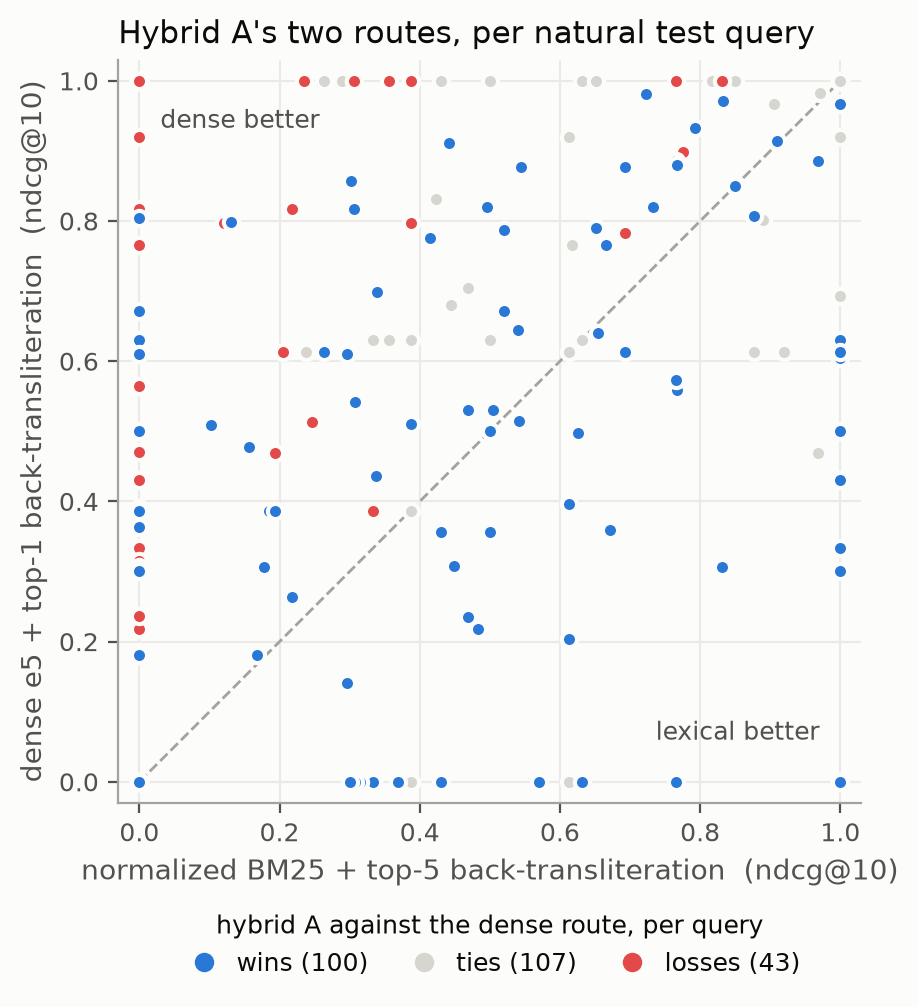
\includegraphics[width=0.48\textwidth]{generated/scatter_components_natural.png}\hfill
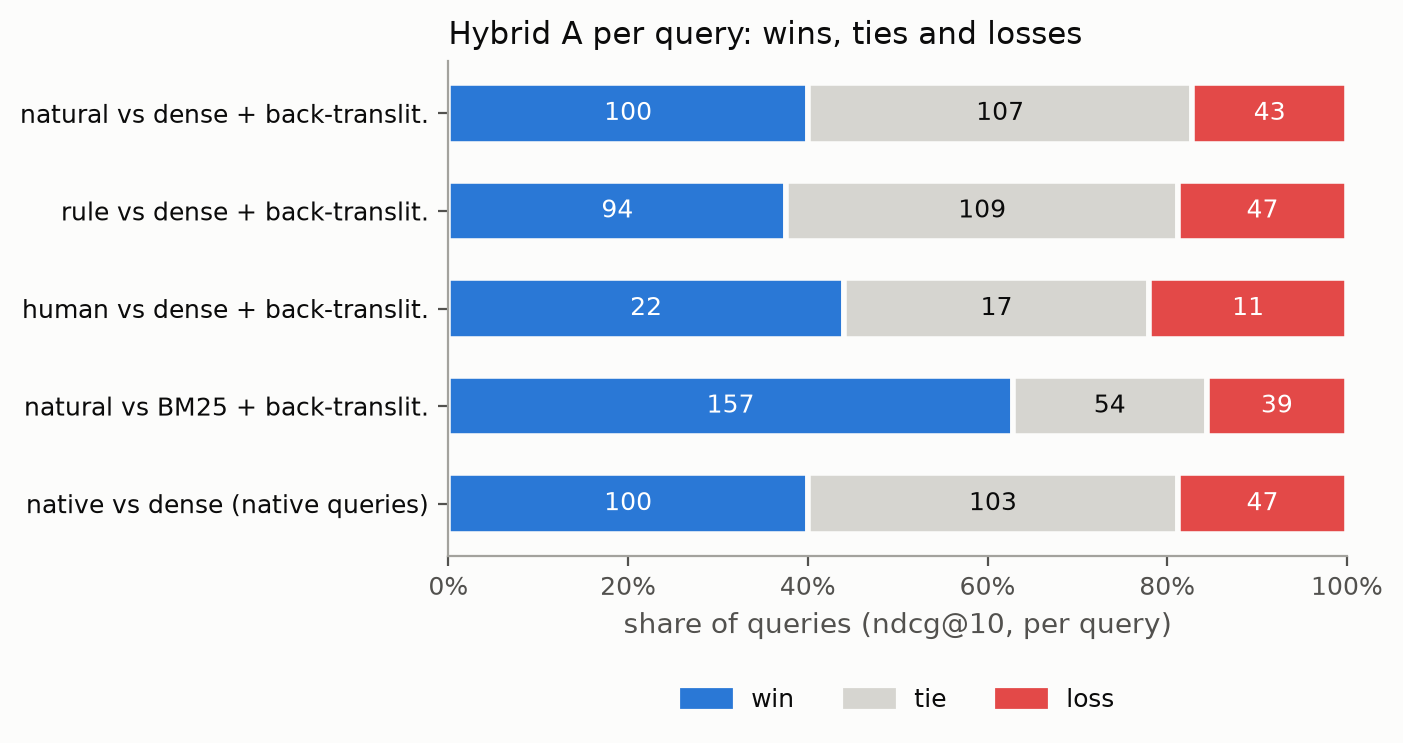
\includegraphics[width=0.50\textwidth]{generated/wins_ties_losses_hybridA.png}
\caption{Left: per natural test query, nDCG@10 of hybrid A's two components, colored by
whether hybrid A beats, ties or loses to the dense component. Right: hybrid A's wins, ties
and losses per query against single methods.}
\label{fig:perquery}
\end{figure}

Figure~\ref{fig:perquery} shows where fusion helps. The lexical route rescues queries on
which the dense route fails (the points along the left and bottom edges), and the hybrid
rarely loses what the dense route had: against dense retrieval it wins 100 natural queries,
ties 107 and loses 43. Long queries gain most: dense retrieval degrades with query length,
BM25 does not.

\paragraph{The final system with native queries.} Hybrid A also helps native queries: 0.6473
against 0.6067 for the dense model ($p < 0.001$). So hybrid A with natural romanized queries
matches the native dense baseline, but stays below the same hybrid with native queries (0.6115
against 0.6473).

\subsection{Gujarati}

\begin{table}[H]
\centering
\caption{Gujarati test results (500 queries), nDCG@10, marks as in Table~\ref{tab:final-hi}
(Bonferroni over 23 comparisons). Every setting was re-chosen on the Gujarati tune split.}
\label{tab:final-gu}
\small
% Generated by scripts/final_table.py --config configs/final_table_gu.yaml; never edit by hand.
\begin{tabular}{llrrr}
\toprule
Phase & Method & native & natural & rule \\
\midrule
10 & BM25 & 0.356$^{-\dagger}$ & 0.013$^{-\dagger}$ & 0.008$^{-\dagger}$ \\
10 & Dense e5 & 0.432 & 0.013$^{-\dagger}$ & 0.002$^{-\dagger}$ \\
10 & BM25 + top-3 back-transliteration & -- & 0.359$^{*}$ & 0.311$^{*}$ \\
10 & Dense e5 + top-1 back-transliteration & -- & 0.337$^{*}$ & 0.296$^{*}$ \\
10 & Normalized BM25 (+ top-3 back-transliteration) & 0.356$^{-\dagger}$ & 0.359$^{*}$ & 0.311$^{*}$ \\
10 & Hybrid A (final system) & 0.494$^{\dagger}$ & 0.474$^{*}$$^{\dagger}$ & 0.429$^{*}$$^{\dagger}$ \\
\bottomrule
\end{tabular}

\end{table}

The gap is just as large in Gujarati (Table~\ref{tab:final-gu}): romanized queries score about
0.01 with both retrievers, against 0.3564 (BM25) and 0.4325 (dense) with native queries.
Back-transliteration again recovers most of it: weighted top-3 BM25 reaches 0.3593 on natural
queries, level with native BM25. Hybrid A ($\alpha = 0.5$) reaches 0.4744 on natural queries,
above the native dense baseline ($\gr = 110\%$), and 0.4938 with native queries. The
normalization key barely matters in Gujarati: only one rule was kept on tune, and it changes
no test result. IndicQA questions share their passage's spelling, so the rules have little to
fix on the native side; likely, IndicXlit's Gujarati output also rarely differs from
Wikipedia's in the variants the rules cover (not measured).

\begin{table}[H]
\centering
\caption{The same methods in both languages: nDCG@10 on test (rank within the language in
brackets) and Kendall's $\tau_b$ between the two rankings. Generated by
\texttt{scripts/compare\_languages.py}.}
\label{tab:compare}
\small
\resizebox{\textwidth}{!}{% Generated by scripts/compare_languages.py --config configs/compare_languages_hi_gu.yaml; never edit by hand.
\begin{tabular}{lrrrrrr}
\toprule
Method & \multicolumn{2}{c}{native} & \multicolumn{2}{c}{natural} & \multicolumn{2}{c}{rule} \\
\cmidrule(lr){2-3} \cmidrule(lr){4-5} \cmidrule(lr){6-7}
 & hi & gu & hi & gu & hi & gu \\
\midrule
BM25 & 0.3810 (4) & 0.3564 (3) & 0.0014 (6) & 0.0129 (6) & 0.0017 (5) & 0.0083 (5) \\
Dense e5 & 0.6067 (2) & 0.4325 (2) & 0.0133 (5) & 0.0134 (5) & 0.0000 (6) & 0.0020 (6) \\
Normalized BM25 (+ top-k back-transliteration) & 0.4040 (3) & 0.3564 (3) & 0.3870 (3) & 0.3593 (2) & 0.3384 (3) & 0.3105 (2) \\
Hybrid A (final system) & 0.6473 (1) & 0.4938 (1) & 0.6115 (1) & 0.4744 (1) & 0.5532 (1) & 0.4287 (1) \\
BM25 + top-k back-transliteration (k = 5 hi, 3 gu) & -- & -- & 0.3737 (4) & 0.3593 (2) & 0.3365 (4) & 0.3105 (2) \\
Dense e5 + top-1 back-transliteration & -- & -- & 0.5608 (2) & 0.3371 (4) & 0.4907 (2) & 0.2963 (4) \\
\midrule
Kendall's $\tau_b$ & \multicolumn{2}{c}{+0.91} & \multicolumn{2}{c}{+0.69} & \multicolumn{2}{c}{+0.69} \\
\bottomrule
\end{tabular}
}
\end{table}

The ranking of methods largely carries over (Table~\ref{tab:compare}; $\tau_b = +0.91$ on
native and $+0.69$ on romanized queries). In both languages hybrid A is first on every query
set and the raw romanized baselines are last. The one swap is in the middle: in Hindi, dense
retrieval with back-transliteration beats lexical top-$k$, in Gujarati lexical top-$k$ is
slightly ahead (0.3593 against 0.3371, not significant). Possible reasons, which we did not
test: e5 is weaker on Gujarati even with native queries (0.4325 against 0.6067), half of the
Gujarati passages are longer than the 256 tokens the model reads, and IndicQA questions share
many words with their passages, which favours BM25. Absolute scores are not comparable
across the two collections (one judged passage per Gujarati question, unjudged distractors);
ranks and $\gr$ are.

% ===========================================================================
\section{Error analysis}

We split the natural Hindi test queries into buckets (Table~\ref{tab:buckets}).

\begin{table}[H]
\centering
\caption{nDCG@10 per bucket of natural Hindi test queries. ``Missed'': native words that
top-1 back-transliteration does not reproduce (after the normalization key). Named entities
were tagged on a 100-query sample.}
\label{tab:buckets}
\small
\begin{tabular}{lrrrrr}
\toprule
Bucket & $n$ & BM25 top-5 norm. & dense top-1 & hybrid A & hybrid A native \\
\midrule
0 words missed   & 144 & 0.3852 & 0.6010 & 0.6410 & 0.6557 \\
1 word missed    & 70  & 0.3832 & 0.5305 & 0.5946 & 0.6433 \\
2+ words missed  & 36  & 0.4015 & 0.4586 & 0.5263 & 0.6212 \\
\midrule
code-mixed       & 57  & 0.3967 & 0.6129 & 0.6212 & 0.6777 \\
no English word  & 193 & 0.3842 & 0.5454 & 0.6086 & 0.6383 \\
\midrule
1--8 words       & 78  & 0.3440 & 0.6290 & 0.6600 & 0.6783 \\
9--12 words      & 106 & 0.4076 & 0.5480 & 0.5846 & 0.6503 \\
13+ words        & 66  & 0.4048 & 0.5006 & 0.5974 & 0.6057 \\
\midrule
named entity     & 47  & 0.5190 & 0.6076 & 0.6646 & 0.7209 \\
no named entity  & 53  & 0.2971 & 0.5085 & 0.5574 & 0.5986 \\
\bottomrule
\end{tabular}
\end{table}

\paragraph{What remains is transliteration error.} When top-1 back-transliteration
reproduces every native word (144 queries), hybrid A is close to its native counterpart
(0.6410 against 0.6557). When it misses two or more words (36 queries), the distance grows
(0.5263 against 0.6212). The weighted lexical query is flat across these buckets: its
alternative candidates absorb the errors, which is why the lexical route helps most where
transliteration fails. Typical errors are short words read as acronyms and the reverse
(\rom{goa} becomes \dev{जीओए}, the letters G-O-A) and names spelled the English way
(\rom{portugal} becomes \dev{पोर्तुगाल}, Wikipedia writes \dev{पुर्तगाल}).

\paragraph{Code-mixing is not the problem.} Queries with an English word score \emph{higher}
with back-transliteration (0.6129 against 0.5454): IndicXlit writes loanwords the way Hindi
Wikipedia does (\dev{डिग्री}).

\paragraph{Named entities help lexical matching; long queries hurt dense retrieval.} Rare
names are highly discriminative terms (BM25: 0.5190 with an entity, 0.2971 without), while
the dense model confuses related entities. Dense quality falls with query length, with native
queries as well, and the hybrid holds up on long queries.

\paragraph{Some losses are judgment artefacts.} MIRACL judges about ten passages per query,
so passages that only the hybrid finds are often unjudged and count as non-relevant; in the
hybrid's largest loss its new first passage is unjudged.

% ===========================================================================
\section{Demonstration}

A Streamlit demo searches either collection with four methods side by side: BM25 with the
query as typed, BM25 with back-transliteration, dense retrieval, and hybrid A. It shows the
back-transliterated query, highlights matched terms, and marks the judged relevant passages
of known queries. Every column is built from the configuration behind a reported run; for the
judged tune queries we checked (one romanized and one native per language), each column's top
10 is identical to the experiment's run file. Words
that do not occur in the experiment queries are back-transliterated live by IndicXlit, which
runs as a small service in its Docker container.

% ===========================================================================
\section{Limitations}

\begin{itemize}
  \item \textbf{Generated queries.} The main romanized set is written by an LLM. It is much
        closer to human typing than Uroman, but has perfect content (no typos or dropped
        words), so the gap real users see may be larger. The hand-typed set has only 50
        queries and one typist, so differences on it are rarely significant.
  \item \textbf{Shallow judgments.} About ten judged passages per Hindi query and one per
        Gujarati query: methods that find new passages are scored as if those were
        non-relevant, and absolute scores are underestimates for every method.
  \item \textbf{Small training set.} Fine-tuning used 1,168 queries, far fewer than the
        reference paper; its effect is bounded by this.
  \item \textbf{One dense model.} Only multilingual-e5-base was used (BGE-M3 did not fit in
        8\,GB for fine-tuning), and no reranker.
  \item \textbf{Gujarati collection.} IndicQA questions were written from their passages,
        and the distractors are unjudged; the Gujarati results show transfer of the method,
        not effectiveness on real Gujarati web search.
  \item \textbf{English-spelled names.} Names typed the English way (\rom{portugal}) cannot be
        back-transliterated reliably, and the LLM prompt asks for exactly that spelling.
\end{itemize}

% ===========================================================================
\section{Future work}

Choosing between top-1 and top-$k$ back-transliteration per word, by IndicXlit's confidence,
could target exactly the queries that still fail. A three-way hybrid (both lexical routes
and dense retrieval) and a reranker on top of the hybrid are natural next steps. Fine-tuning
on back-transliterated training queries, or on more and noisier romanized queries, could make
the dense route robust to transliteration errors. Finally, a test set of queries typed by
several real users, with deeper judgments, would show the gap as users experience it.

% ===========================================================================
\section{Conclusion}

The script gap is real and near-total for both lexical and dense retrieval in Hindi and
Gujarati. Fine-tuning the retriever on romanized queries closes only part of it; rewriting
the query into native script closes most of it with off-the-shelf components, and fusing
normalized BM25 with dense retrieval on the rewritten query closes the rest on natural
romanized queries. The same recipe transfers to Gujarati with its settings re-chosen on tune.
What remains is transliteration error on a minority of queries, mostly acronyms and names
spelled the English way.

\bibliographystyle{plainnat}
\bibliography{references}

\end{document}
